\chapter{Практика}\label{ch:ch3}

\section{Мобильный автономный робот}
Для решения задачи данной работы необходимо было проводить <<живые>> тестирования работы алгоритмов. Такая необходимость обусловлена прежде всего тем, что помимо существующей задачи данной ВКР стояла задача в создании робота для распознавания объектов. По этой причине было принято решение делать алгоритмы на реальном роботе\footnote{Задание данной ВКР можно было бы сделать и в любом симуляторе или игровом движке. Однако решение делать всё в реальной жизни сильно усложнило данную задачу.} с пребыванием данного робота во вполне реальных условиях.

\subsection{Подбор шасси}
Как было сказано в \fixme{первой} главе данной работы, существует большое количество различных шасси, на которых можно располагать различное оборудование. Наш выбор остановился на гусеничном шасси TS100, заказанном с платформы AliExpress, которое изображено на Рисунке~\ref{fig:ts100}.

%https://aliexpress.ru/item/32879237800.html
\begin{figure}[ht]
  \centerfloat{
    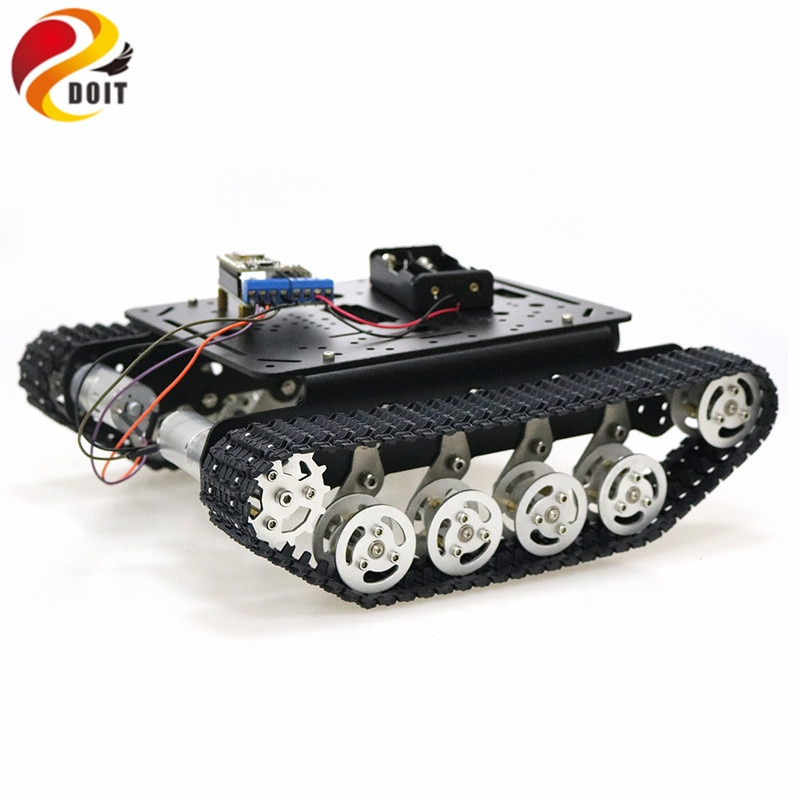
\includegraphics[scale=0.6]{ts100}
  }
  \caption{Шасси TS100 для самодельного робота.}\label{fig:ts100}
\end{figure}

Данное шасси за счёт своих размеров является очень мобильным средством передвижения робота и может проникнуть в относительно узкие для роботов пространства и без проблем оттуда выбраться, не повредившись. Для дополнительного оборудования на данном шасси место тоже нашлось: для этого было принято решение заказать дополнительную металлическую пластину, которая в последствии роль сыграла второго этажа. Шасси с уже установленным вторым этажом можно увидеть на Рисунке~\ref{fig:robot-empty}.

\begin{figure}[ht]
  \centerfloat{
    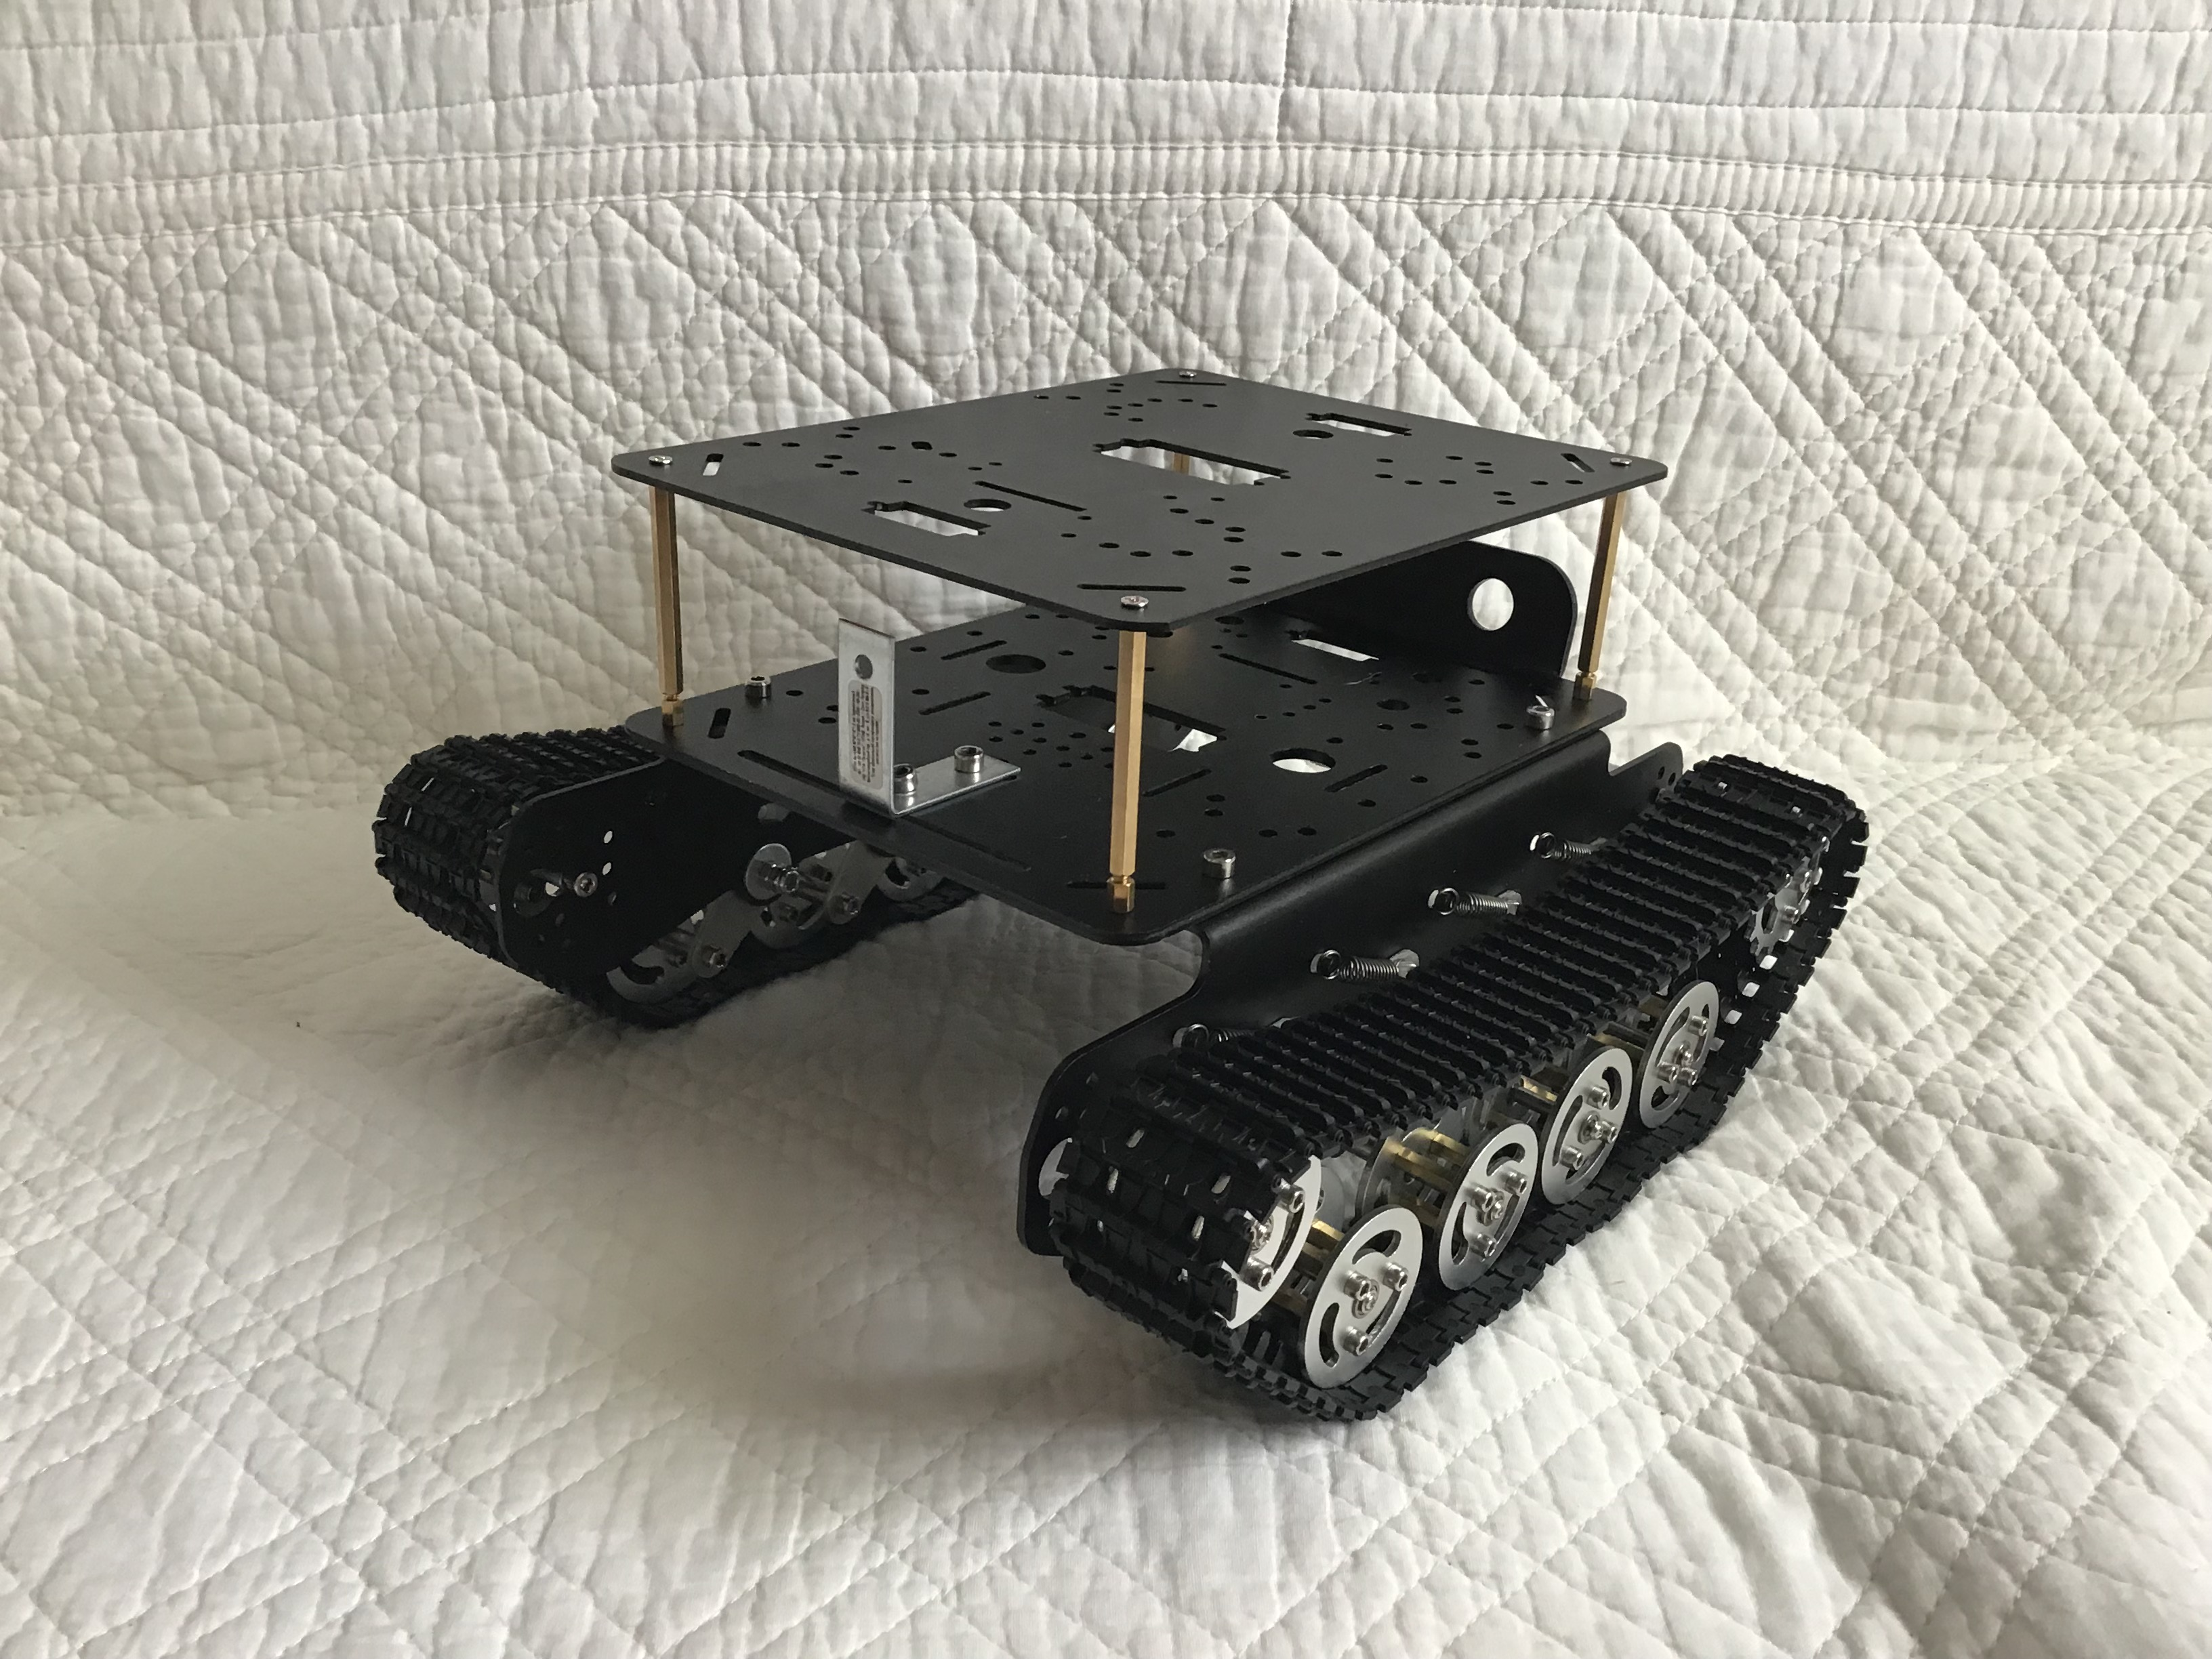
\includegraphics[scale=0.1]{robot-empty.jpeg}
  }
  \caption{Шасси робота без установленного на него оборудования.}\label{fig:robot-empty}
\end{figure}

\subsection{Движение шасси} \label{sub:robot-move}

К сожалению, по неизвестной причине к данному шасси не пришёл комплектный контроллер движения, который бы принимал команды от компьютера и заставлял двигаться два электродвигателя, установленные на шасси. Поэтому пришлось немного изучить ещё одну предметную область, которая не изучалась в течении университетского курса - электротехнику. 

\subsubsection{Контроллер двигателей}

Компьютер, который будет в последствии установлен на робота будет управлять роботом посредством сигналов с напряжением 3.3В через порт GPIO, где 0 (или по-другому нет напряжения) - это движение не требуется и 1 (когда есть напряжение +3.3В), когда движение требуется.

Контроллер должен, также, уметь по отдельности управлять двумя гусеницами, заставлять их ездить вперёд и назад. Не мало важна и компактность решения, и энергоэффективность. Это основные требования. Из дополнительных требований можно выделить умение каким-то образом регулировать скорость движения. Общая структура желаемой модели контроллера изображена на Рисунке~\ref{fig:structure-controller}. 

\begin{figure}[ht]
  \centerfloat{
    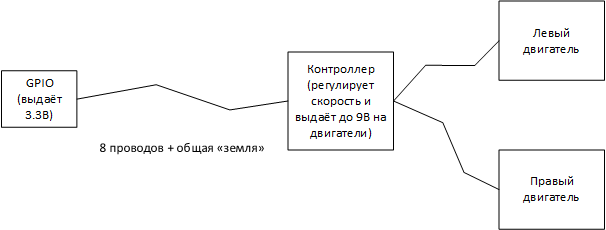
\includegraphics[scale=0.9]{structure-controller.png}
  }
  \caption{Общая структура желаемой модели контроллера.}\label{fig:structure-controller}
\end{figure}

Таким образом спустя пару экспериментов с текстолитом и монтажными платами получился полноценный контроллер, который умеет управлять роботом с медленной и быстрой скоростями, однако у него были свои сильные недостатки речь о которых в данной ВКР не зайдёт. Получившийся контроллер изображён на Рисунке~\ref{fig:robot-controller}.

\begin{figure}[ht]
  \centerfloat{
    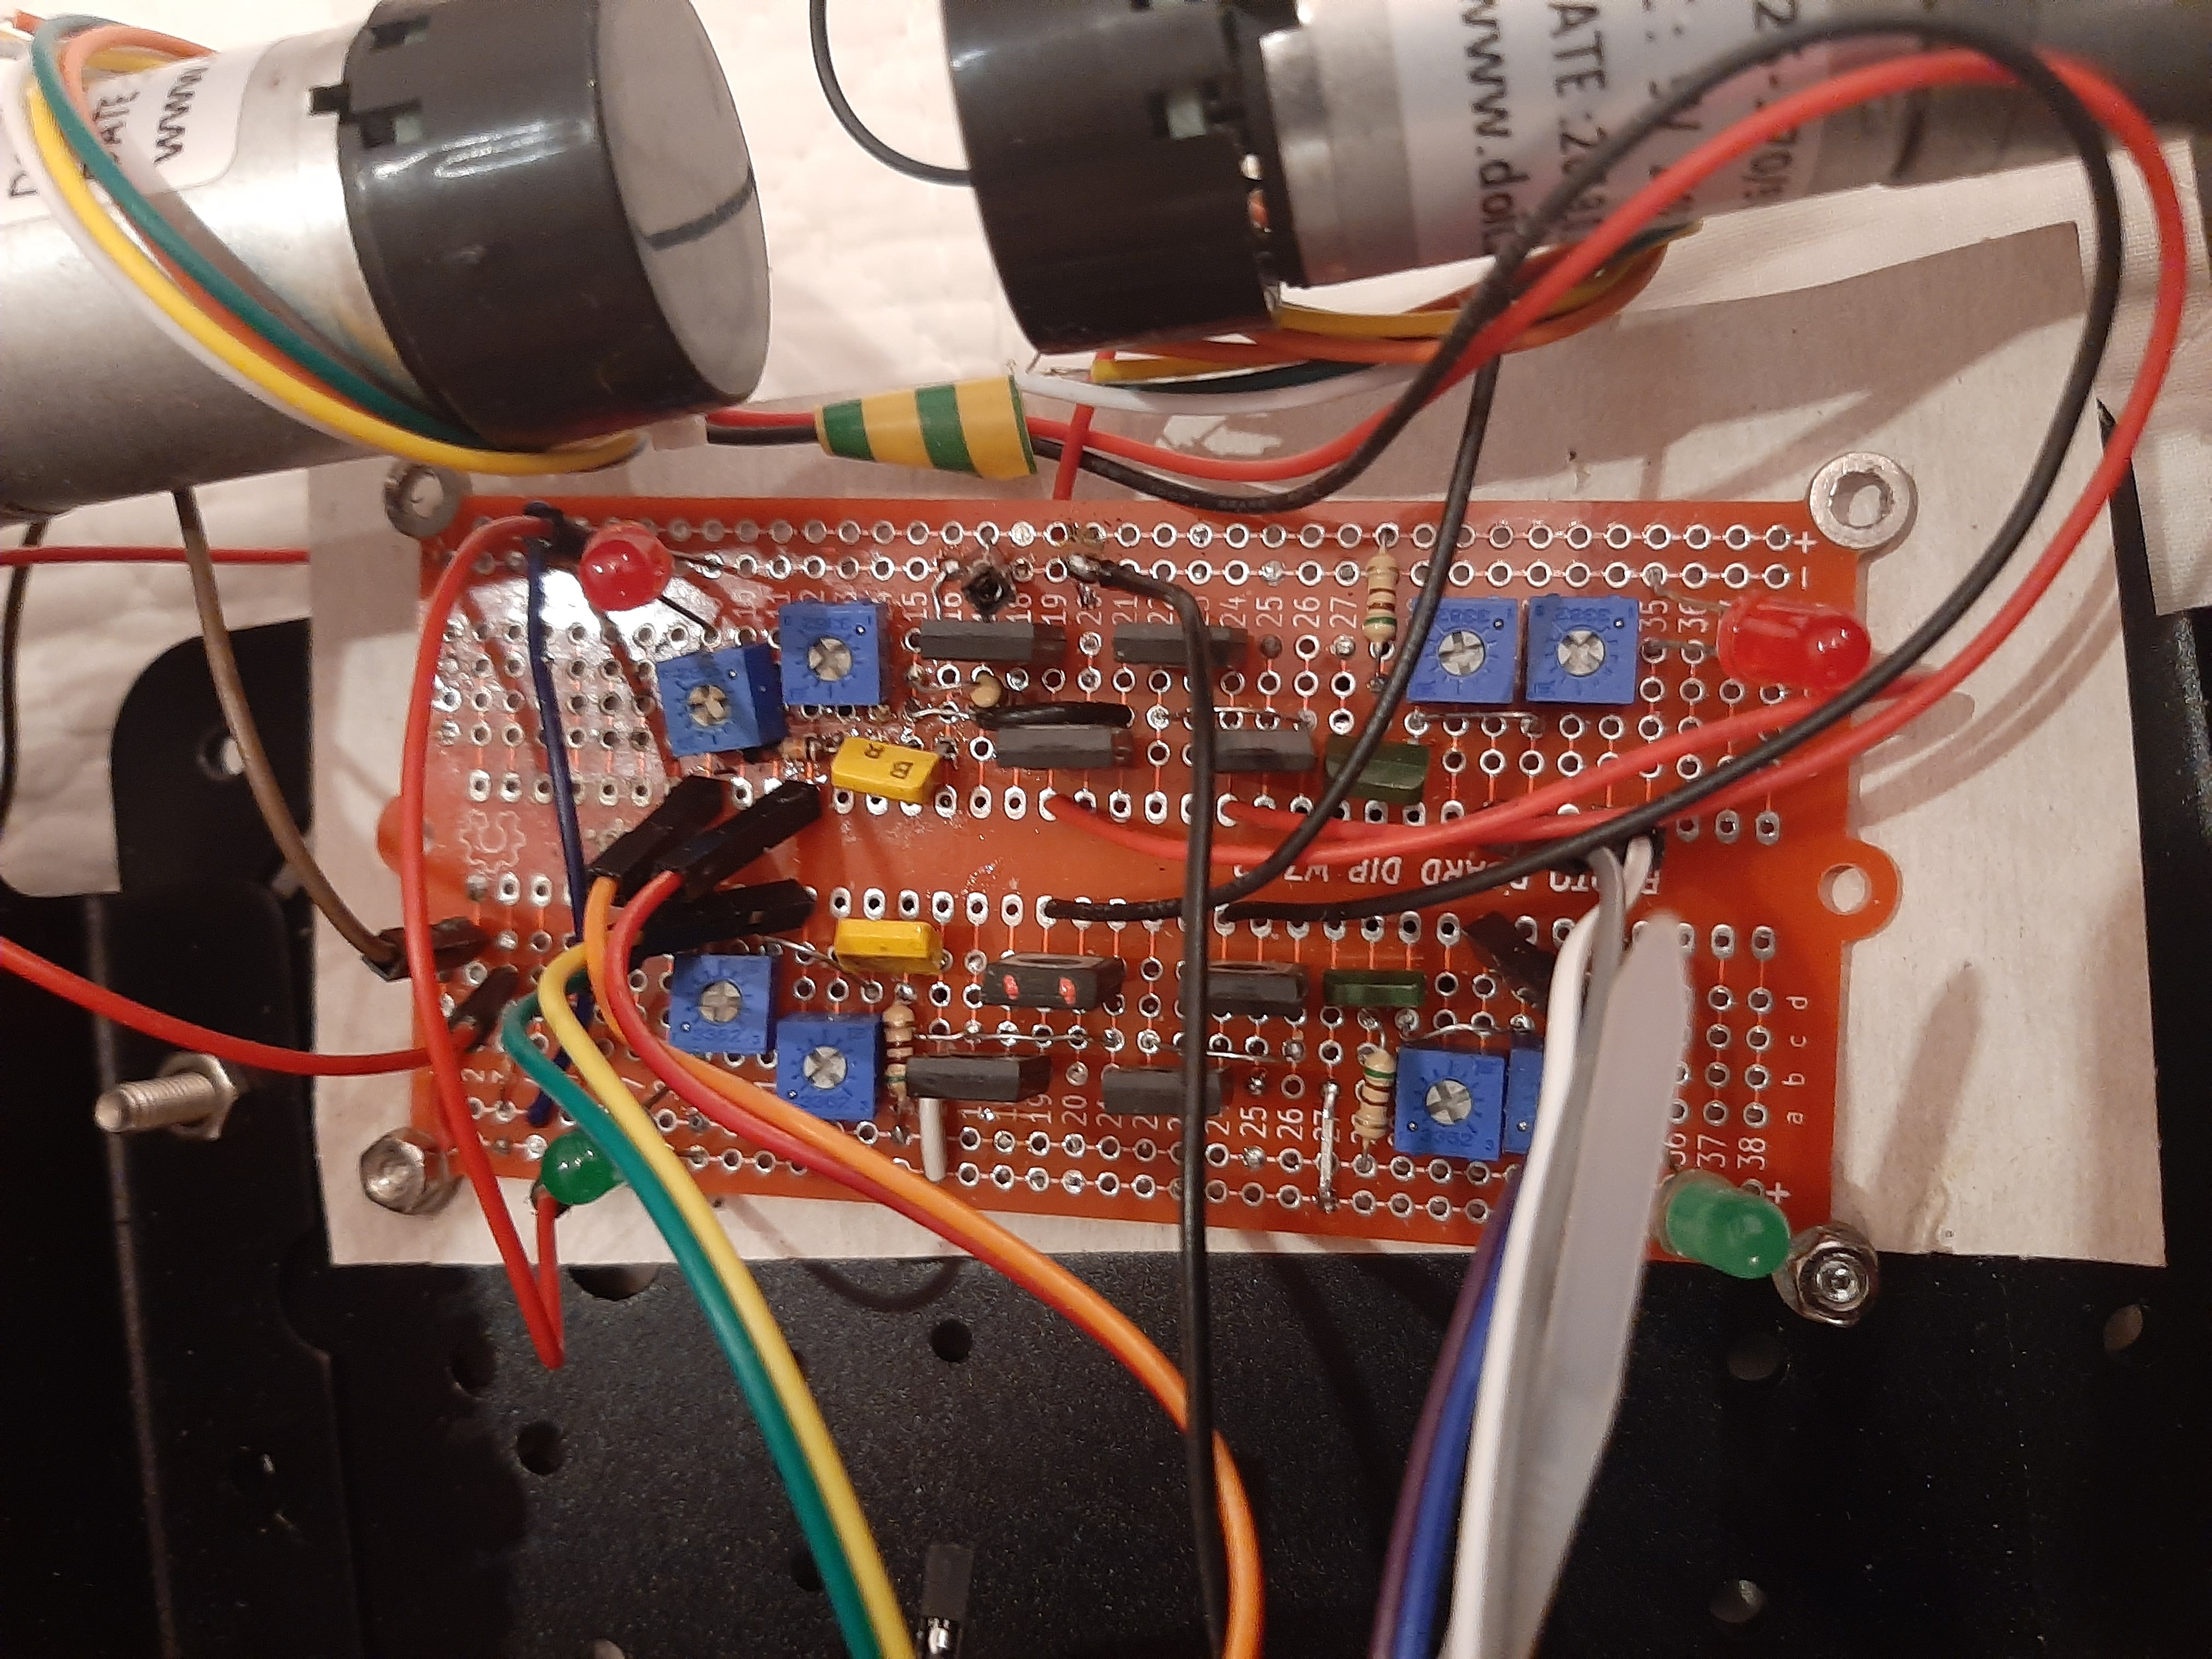
\includegraphics[scale=0.1]{robot-controller.jpg}
  }
  \caption{Готовый экземпляр контроллера двигателей.}\label{fig:robot-controller}
\end{figure}

\section{Визуальный анализ пространства}
Для анализа окружающего пространства существует довольно большое количество различных датчиков и прочего оборудования \fixme{пруф}. Но закупать сразу всё не выгодно экономически, затратно в плане места размещения на роботе и расточительно в плане потребления электроэнергии этими самыми датчиками. Также для обработки всех этих сигналов нужны соответствующие вычислительные мощности. 

Таким образом робот должен иметь совсем небольшое количество сенсоров и при этом не быть <<слепым>>. Исходя из этих соображений, было решено установить на робота два основных сенсора: лазерный сканер YDLIDAR X4 (изображён на Рисунке~\ref{fig:ydlidar-x4}) и CSI камеру Sony IMX219 (изображена на Рисунке~\ref{fig:imx219}). Первый поможет видеть препятствия вокруг робота, второй сможет <<видеть>> целевые объекты, размещённые перед роботом. 

%https://www.ydlidar.com/products/view/5.html
%https://aliexpress.ru/item/4000112261464.html
\begin{figure}[ht]
    \centerfloat{
        \hfill
        \subcaptionbox[List-of-Figures entry]{2D лидар YDLIDAR X4.\label{fig:ydlidar-x4}}{%
            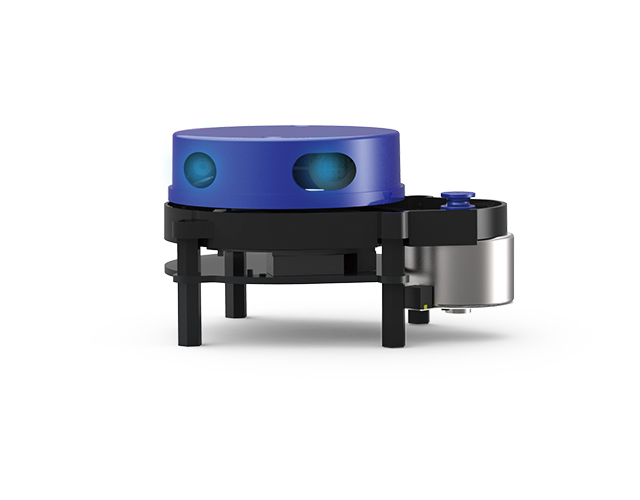
\includegraphics[width=0.5\linewidth]{ydlidar-x4}}
        \hfill
        \subcaptionbox{CSI камера с сенсором Sony IMX219. \label{fig:imx219}}{%
            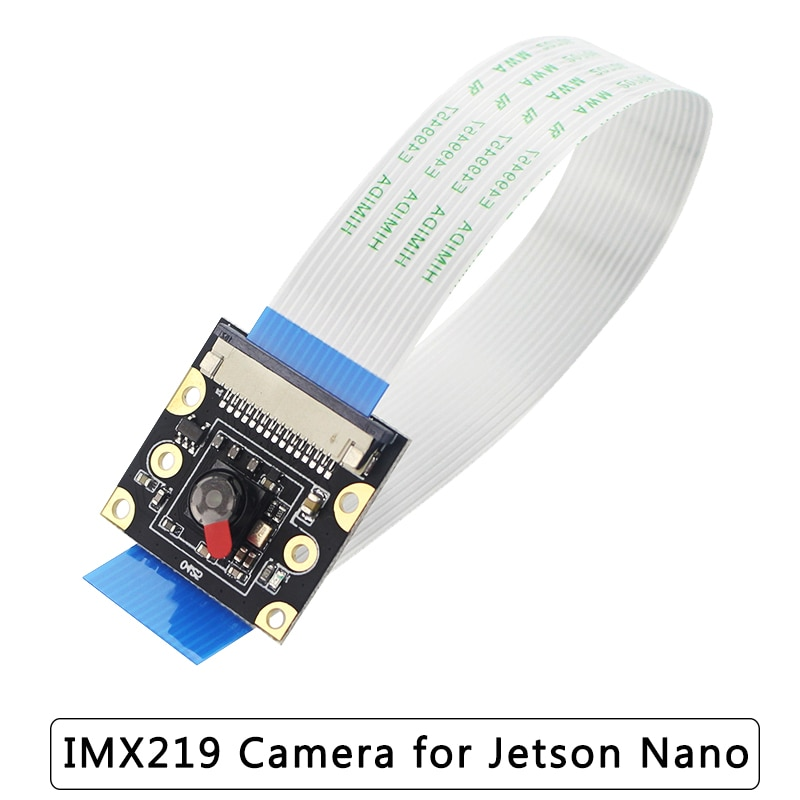
\includegraphics[width=0.4\linewidth]{imx219}}
        \hfill
    }
\end{figure}

%Схема размещения сенсоров \fixme{приведена на Рисунке }.

\section{Формирование поведенческой стратегии робота}

Основная задача робота - ездить и искать целевые объекты делится на две подзадачи: исследование пространства и подъезд к целевому объекту.

\subsection{Исследование пространства}

Данный режим будет подразумевать под собой то, что робот будет просто ехать вперёд, параллельно разыскивая целевые объекты и объезжать возникшие перед ним препятствия. 

\subsubsection{Объезд препятствий} \label{subsub:obstacle-avoidance}

Робот должен уметь объезжать хотя-бы самые простейшие препятствия, по типу стен, диванов или прочих перегородок. В идеале, он должен уметь справляться и с тонкими препятствиями по типу ножек стула и мягкие поверхности.

Алгоритм объезда препятствий, представленный на данном роботе сводится к схеме, изображённой на Рисунке~\ref{fig:algorithm-obstacle}.

\begin{figure}[ht]
  \centerfloat{
    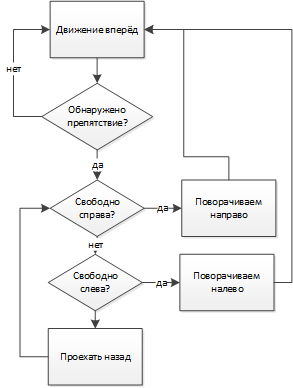
\includegraphics[scale=0.9]{algorithm-obstacle.png}
  }
  \caption{Общая схема алгоритма объезда препятствий.}\label{fig:algorithm-obstacle}
\end{figure}

Подсчёт того, где свободнее: слева или справа идёт из соображений того, где находится больше препятствий. Как это считается? Условно робот поделён на несколько направлений. В данном случае он подразделён на <<перед>>, <<лево>>, <<право>> и <<зад>>. Обозначим значения, которые подсчитываются на этих направлениях, как $f, l, r$ и $b$ соответственно. 

Лидар выдаёт данные в формате массива значений float: обозначим его как числовой ряд $a$. В этом числовом ряду находятся числа, обозначающие расстояние до точки об которое отразился лазер. Чем больше число, тем дальше находится объект об который отразился лазер. Если лазерный сканер не нашёл в этом месте отражения, то он возвращает значение -1. Фактически, данный массив является аналогом полярных координат, где позиция значения в массиве - это угол, а само значение является расстоянием. Всего этих чисел 720, из чего можно сделать вывод, что цена деления лидара это полградуса. 

Таким образом каждый поворот лидара вычисляются 4 переменные\footnote{Важное замечание: значения -1, когда лазерный сканер не нашёл отражения заменяются на значение 1 для того чтобы значения переменных прибавлялись, а не уменьшались.}:

\[
\begin{array}{c}
l = \frac{\displaystyle\sum_{i=90}^{270} a_i}{180} \quad
b = \frac{\displaystyle\sum_{i=270}^{450} a_i}{180}\quad
r = \frac{\displaystyle\sum_{i=450}^{630} a_i}{180} \quad
f = \frac{\displaystyle\sum_{i=630}^{720} a_i + \sum_{i=0}^{90} a_i}{180}
\end{array}
\]

После вычисления этих средних арифметических значений по каждой из сторон проверяются значения массива $a_i$, где $630 < i < 720$ и $0 < i < 90$ (передняя сторона робота) и если среди этих чисел находится хоть одно удовлетворяющее условию $0 < a_i < 0,3$, то считается в данный момент перед роботом находится какое-то препятствие.

Если это так, то далее сравниваются значения ранее высчитанных переменных $l$ и $r$. Если значение $l > r$, то робот поедет налево, так как слева нашлось меньше препятствий, чем справа. Иначе, роботу следует ехать направо. Однако представленного выше алгоритма ещё недостаточно чтобы объезжать часто встречаемые препятствия. 

\subsubsection{Обнаружение застревания}

Робот может попасть в ситуацию, когда впереди внезапно образовалась преграда, невидимая для лазерного сканера (например, очень низкая преграда). Для обнаружения застревания при столкновении с такими преградами необходимо как-то понять, что робот перестал двигаться. 

Одним из способов понять и распознать застревание может стать анализ облака точек, которые выдаёт LIDAR. Если вектор движения большинства точек на плоскости облака стал достаточно мал, то можно сделать вывод о том, что робот либо плохо двигается, либо вообще застрял. 

В данный проект была встроена система Google Cartographer, которая по облаку точек может строить окружающую карту местности (пример такой карты изображён на Рисунке~\ref{fig:cartographer-example}), а также определять местоположение робота на ней \fixme{вставить цитату в которой это подтверждается}. Информацию о местоположении можно использовать как раз в целях определения застревания. Если в течении секунды координаты робота менялись недостаточно сильно, значит робот застрял.

\begin{figure}[ht]
  \centerfloat{
    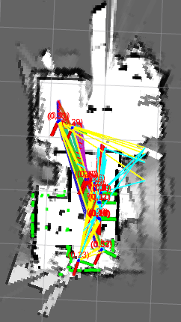
\includegraphics[scale=0.8]{cartographer-example}
  }
  \caption{Пример карты, сгенерированной Google Cartographer.}\label{fig:cartographer-example}
\end{figure}

Для выезда из застревания используется простой алгоритм, который состоит из 3 шагов:

\begin{enumerate}
\item Ехать назад 2 секунды;
\item Выбрать сторону, в которую будет совершён поворот по значениям выше упомянутых переменных $l$ и $r$;
\item Ехать дальше.
\end{enumerate}

Как показала практика, этот алгоритм, работает достаточно эффективно для того чтобы не застревать в большинстве ситуаций.

\subsection{Подъезд к целевому объекту}

Данный режим предполагается включать только в случае, если на видеосигнале, получаемом от CSI камеры был распознан целевой объект. В этом случае робот останавливается и поворачивается в ту сторону, где расположен центр предполагаемого целевого объекта. Далее робот начинает ехать вперёд и по мере необходимости продолжает центрировать шасси до тех пор пока не подъедет к объекту. Далее робот останавливается, конечная цель робота выполнена: целевой объект найден. 

Определение того, что робот подъехал к объекту происходит по размеру прямоугольника, на котором обозначен целевой объект. Если прямоугольник уже достиг краёв кадра видеосигнала, значит робот приблизился к объекту максимально близко. Подъезд вплотную к объекту является не самой лучшей идеей, так как целевым объектом может быть стеклянная бутылка, которую можно просто сбить и разбить.

\section{Подробнее о программной части робота}
На одноплатный компьютер Nvidia Jetson Nano была установлена операционная система Ubuntu LTS 18.04 со специальным от Nvidia программным обеспечением JetPack 4.3, которое предоставляет удобные инструменты для вычислений в области искусственного интеллекта при помощи встроенного в Jetson NANO видеочипа и ядер CUDA. Также на компьютер была установлен фреймворк для программирования роботов ROS, аббревиатура которого расшифровывается как <<Операционная система для роботов>>.

\subsection{ROS}
\fixme{Свистнуть все ссылки с преддипломки}
ROS предоставляет удобные и мощные функции, помогающие разработчикам в таких задачах, как передача сообщений различного типа, распределение вычислений между компьютерами, повторное использование кода и реализация современных алгоритмов для роботизированных приложений. В общем случае, ROS представляет собой инструмент, позволяющий связывать несколько независимых программных модулей при помощи сервисов и узлов, которые могут передавать друг другу сообщения в различном формате. Структура ROS представлена на Рисунке \ref{fig:ros-compute-graph}.

%Притянуто из книжки по ROS
\begin{figure}[ht]
  \centerfloat{
    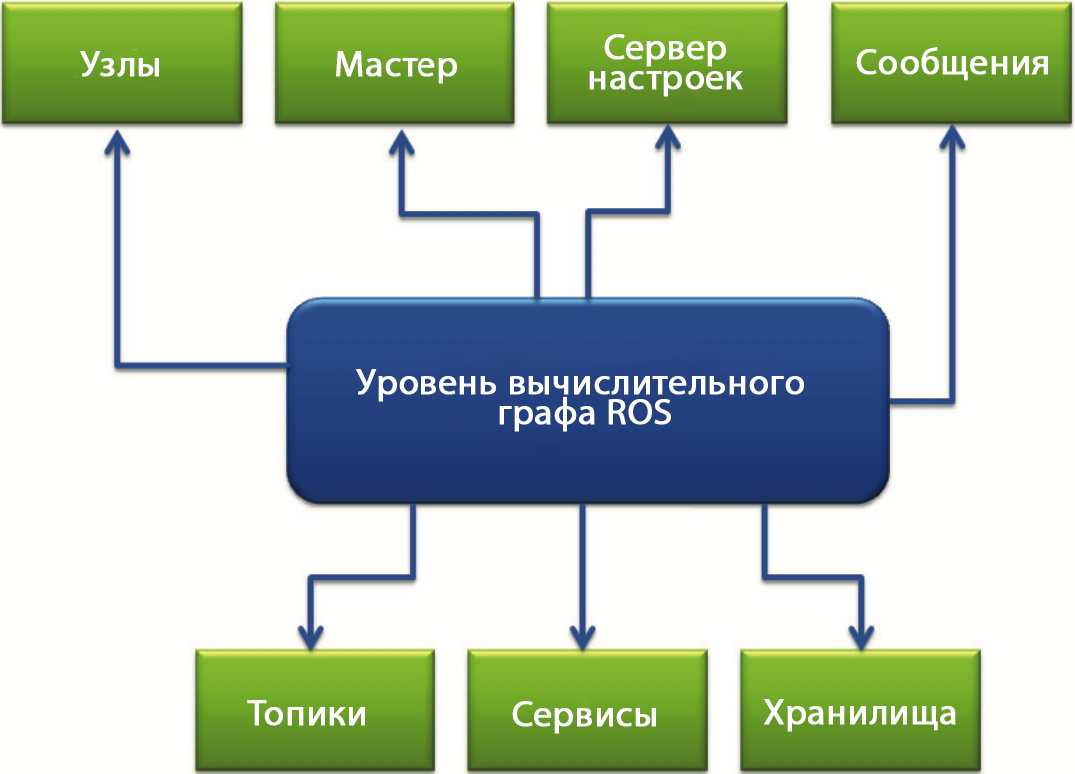
\includegraphics[scale=0.3]{ros-compute-graph.png}
  }
  \caption{Общая структура Robot Operating System.}\label{fig:ros-compute-graph}
\end{figure}


Большими преимуществами использования данного фреймворка является возможность передачи сообщений по локальной сети и обширная библиотека уже реализованного ПО, которое можно без относительно больших затрат по времени интегрировать в свой собственный проект. На момент написания данной ВКР глобальный репозиторий ROS Index насчитывает 2120 подключенных к нему сторонних репозиторием и 5827 пакетов. Диаграмму соответствия пакетов в репозитории с версиями ROS можно увидеть на Рисунке~\ref{fig:ros-index}\footnote{Версия, используемая на роботе - Melodic}.

%https://index.ros.org/stats
\begin{figure}[ht]
  \centerfloat{
    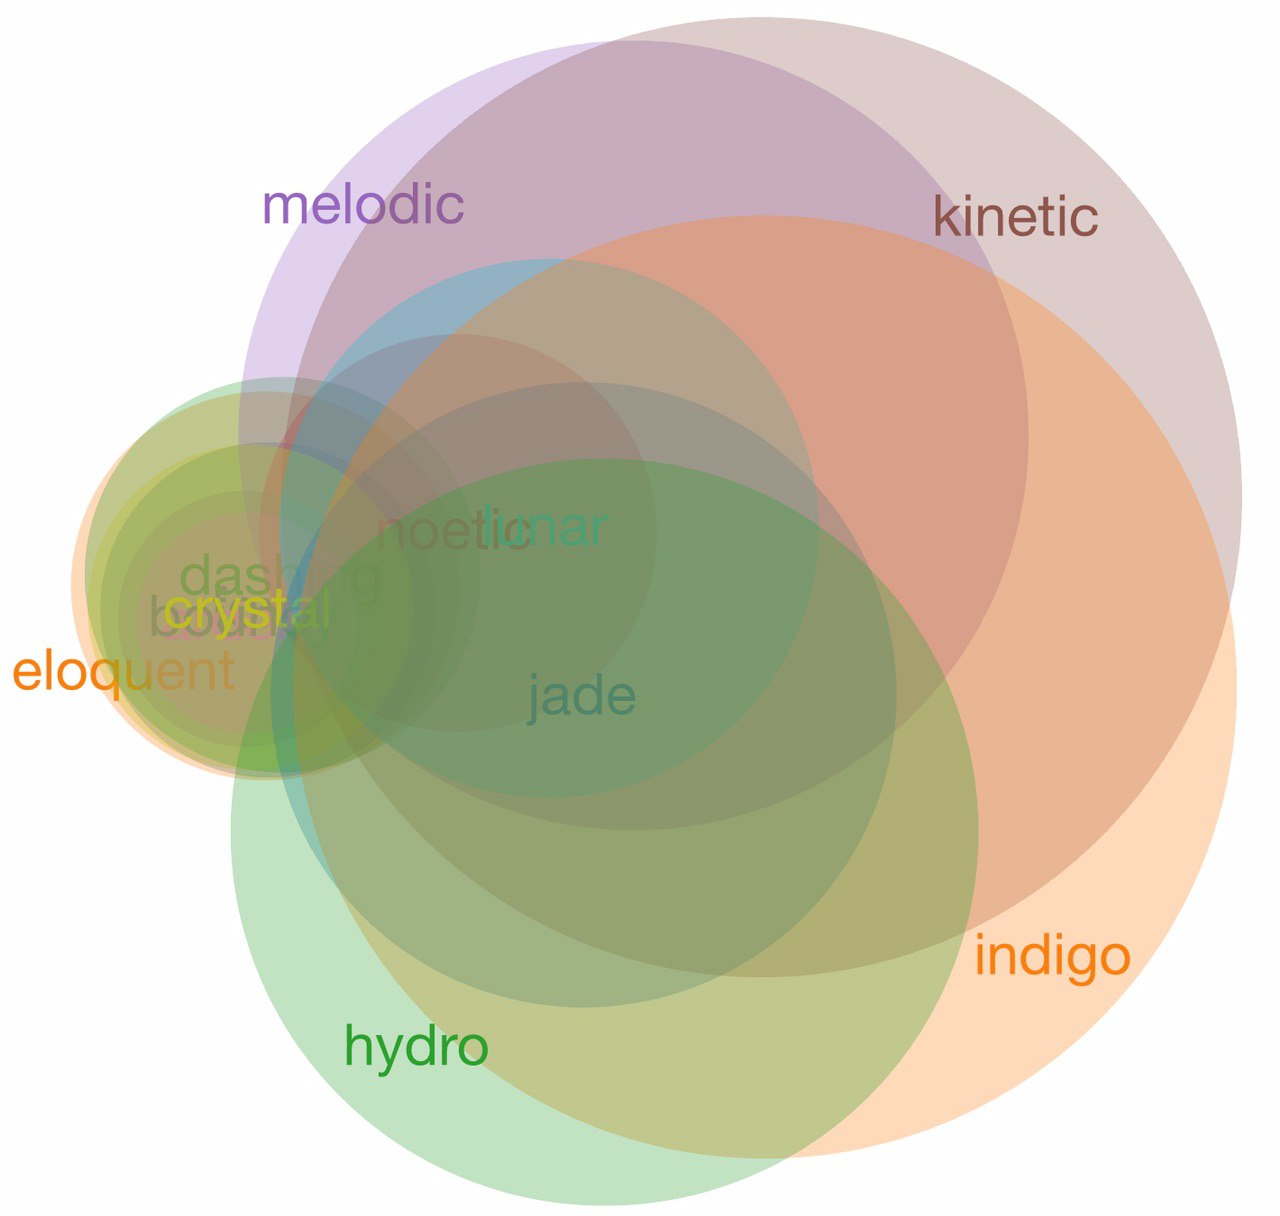
\includegraphics[scale=0.2]{ros-index}
  }
  \caption{Глобальный репозиторий ROS Index и версии ROS.}\label{fig:ros-index}
\end{figure}

\subsection{Концепции ROS}
Ниже приведён список концепций рассматриваемого фреймворка \fixme{ссылки с преддипломки}:
\begin{itemize}
\item {\textbf{Узел} - это процесс, выполняющий вычисления. Каждый узел написание с использованием клиентских библиотек ROS. Используя методы связи, узлы могут общаться друг с другом заранее определённым форматом сообщений и обмениваться данными. Для этого создаются узлы-подписчики, и узлы-публикаторы.}
\item {\textbf{Мастер} - обеспечивает регистрацию и работоспособность запущенных узлов.}
\item {\textbf{Сообщение} - простая структура данных, содержащая типизированное поле, которое может содержать целый набор данных, отправляемых на другой узел. Помимо стандартных типов сообщений\footnote{Такие как целые, с плавающей точкой, логические, строковые...} возможна отправка заранее обозначенных собственных типов сообщений.}
\item {\textbf{Тема} - именованная шина данных, используемая узлами для отправки сообщений. Публикующий и подписанный узел не знают о существовании друга друга. Благодаря тому что каждая тема имеет уникальное имя, любой узел может получить доступ к данной теме и отправляет через неё данные, при условии соблюдении заранее оговорённых передаваемых типов, данной темой.}
\item {\textbf{Сервисы} - реализация удалённого вызова процедур\footnote{RPC} в ROS. В некоторых случаях модель связи публикации и подписки может не подходить. В этих случаях и применяют взаимодействия в виде сервисов (схема запрос/ответ), при котором один узел может запросить выполнение процедуры для другого узла, ожидая какого-то обязательного ответа\footnote{В случае использования схемы с подписчиками и публикаторами доставка сообщений и ответ не гарантируются}.}
\end{itemize}

\subsection{Узлы, используемые на роботе}
В рамках работы над данной ВКР были реализованы следующие узлы и сервисы:
\begin{itemize}
\item Сервис, управляющий сигналами на разъёме GPIO; 
\item Узел записи видео с видеокамеры;
\item Узел распознавания объектов;
\item Узел, управляющий движением робота и формирующий поведенческую стратегию робота.
\end{itemize}

Также в роботе используются следующие сторонние узлы:
\begin{itemize}
\item Узел передачи изображения с CSI видеокамеры;
\item Google Cartographer;
\item Узел YDLIDAR.
\end{itemize}


Общую схему взаимодействия всех узлов можно увидеть на Рисунке~\ref{fig:rosgraph}.

\begin{figure}[ht]
  \centerfloat{
    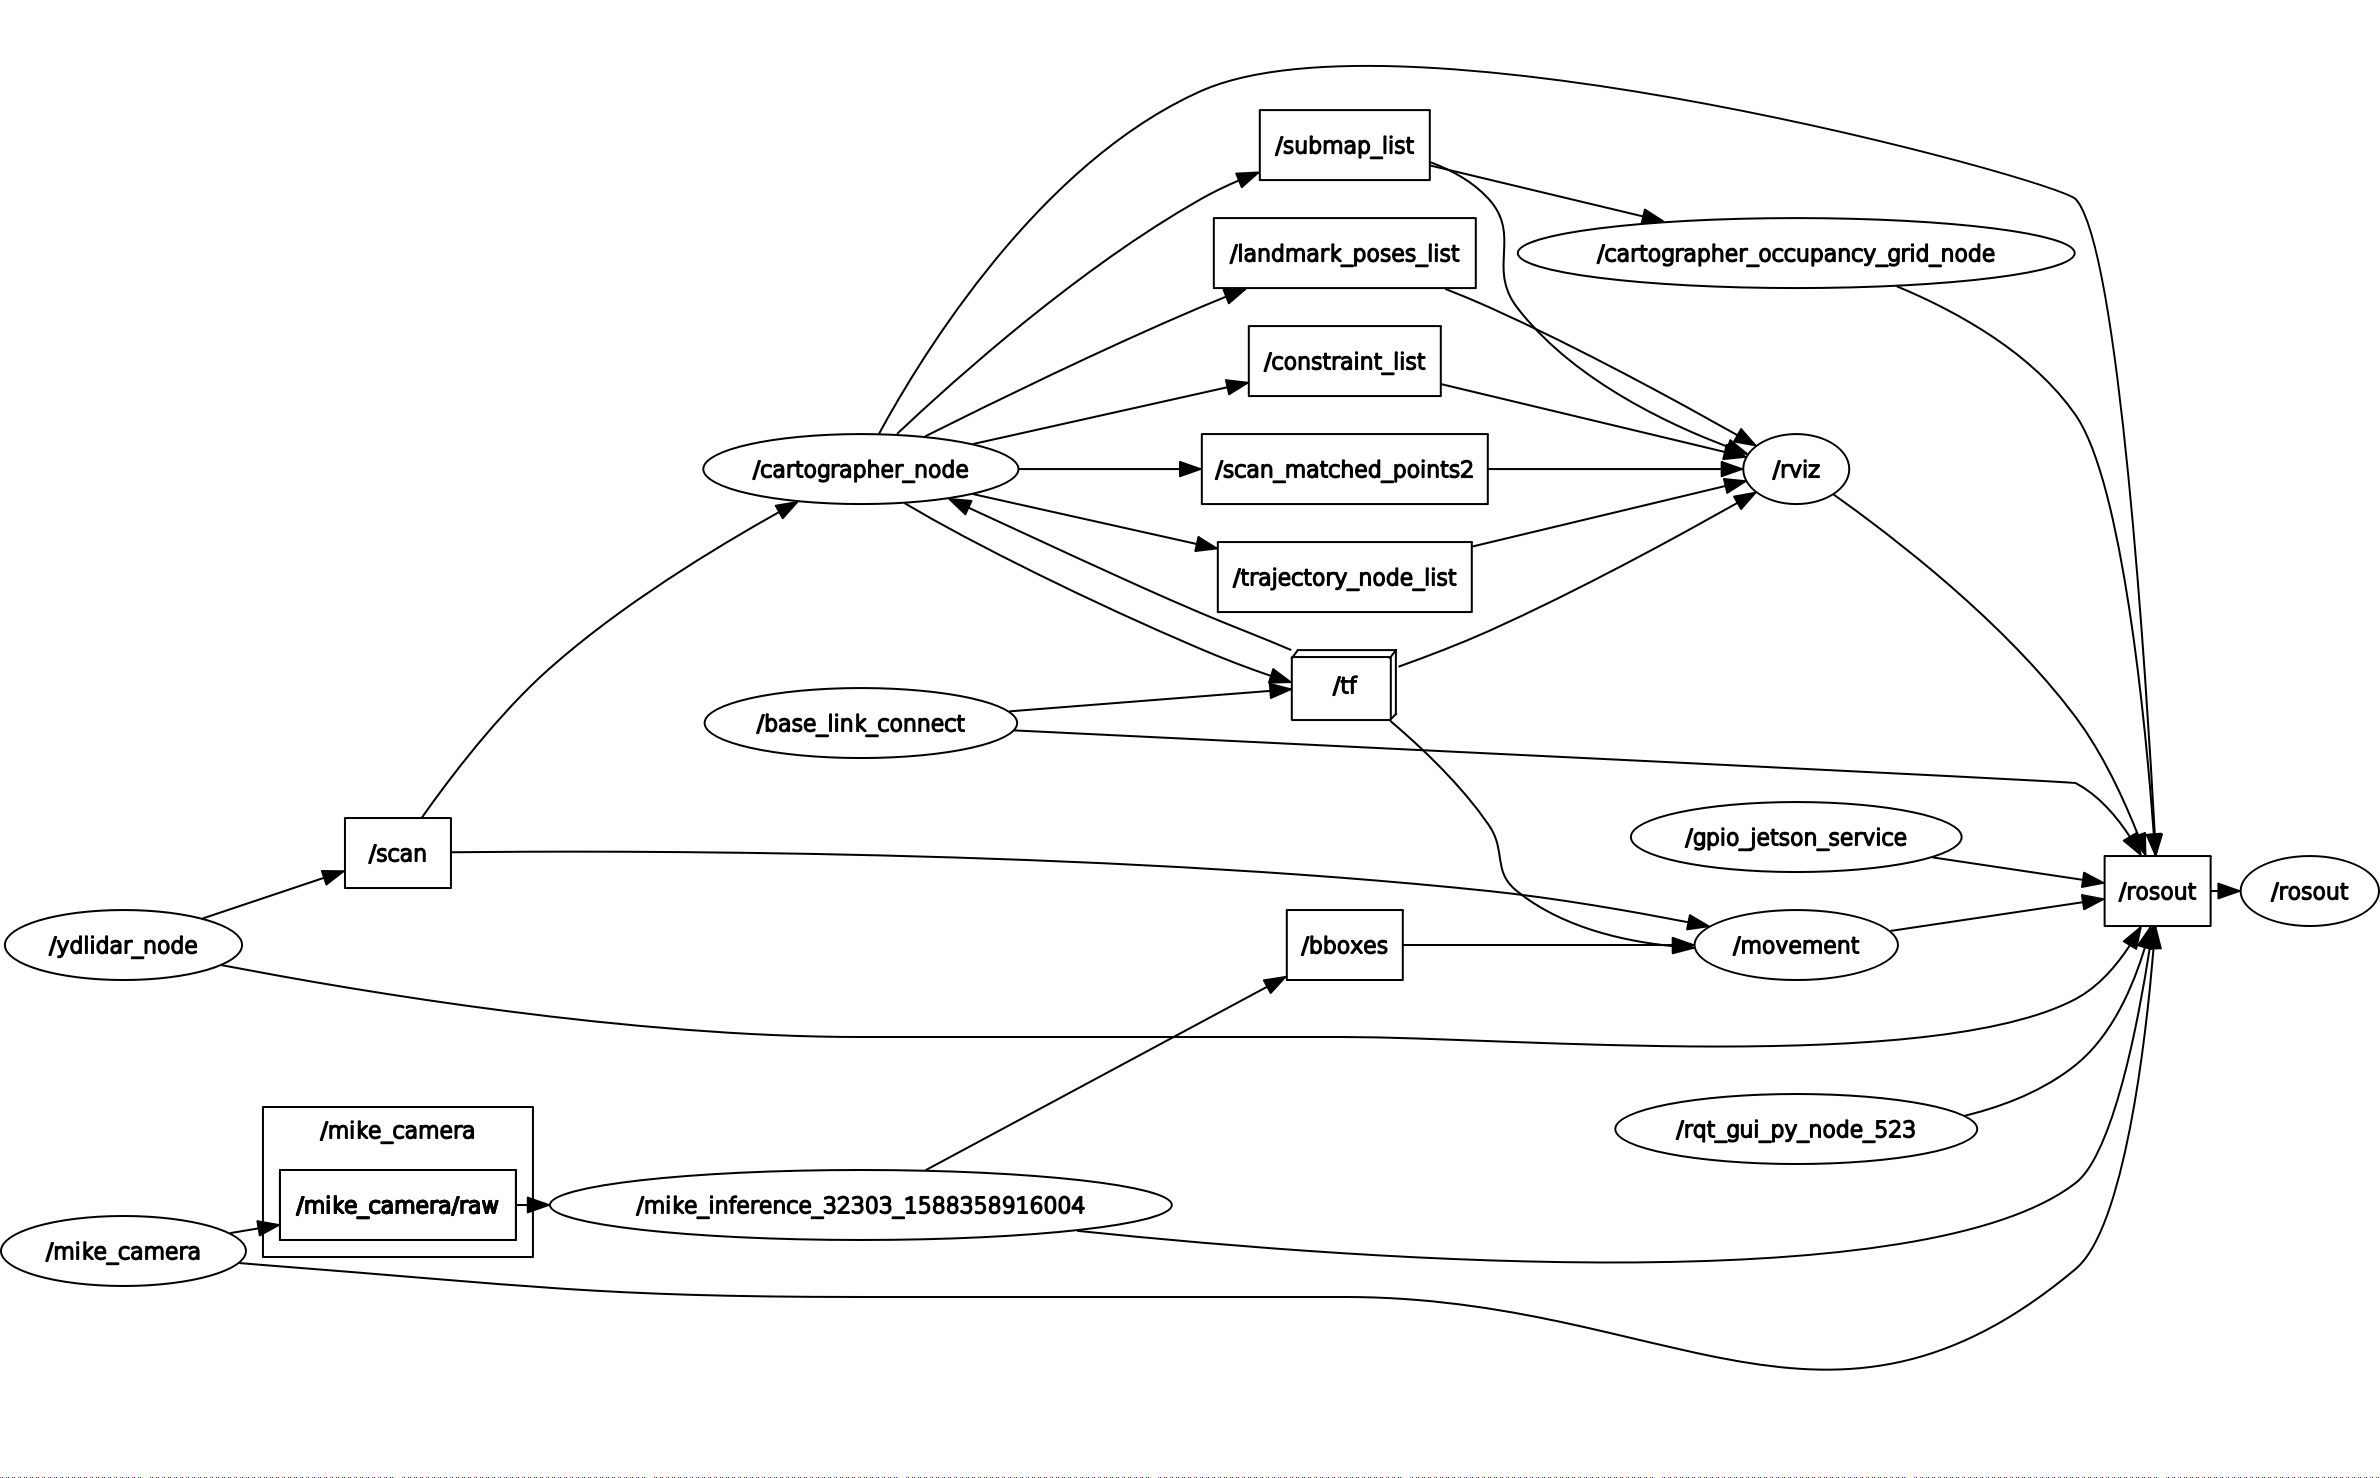
\includegraphics[scale=0.25]{rosgraph.png}
  }
  \caption{Общая схема взаимодействия всех узлов и сервисов робота, сгенерированная ROS Graph.}\label{fig:rosgraph}
\end{figure}

\subsubsection{Узел видеокамеры}
Данный узел был заимствован из репозитория робота JetBot и он публикует изображения в формате сообщения, описанного стандартом ROS sensor\_msgs/Image (содержание сообщения можно \fixme{увидеть в Приложении }), получаемые из CSI камеры IMX219, подключенной к Nvidia Jetson NANO. 

Для получения такого видеосигнала используется библиотека GStreamer и встроенные в образ Linux драйвера на данный сенсор. Пример получаемого изображения показан на Рисунке~\ref{fig:robot-camera-test}.

\begin{figure}[ht]
  \centerfloat{
    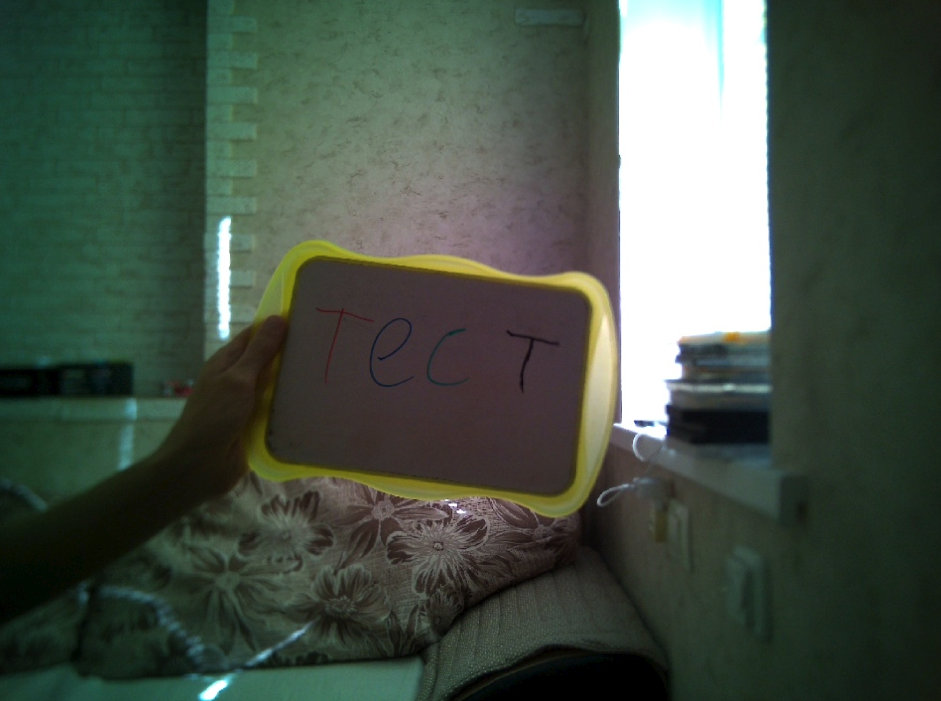
\includegraphics[scale=0.4]{robot-camera-test.png}
  }
  \caption{Пример получаемого изображения с CSI камеры Sony IMX219.}\label{fig:robot-camera-test}
\end{figure}

Таким образом на выходе данного узла получается топик по имени raw, содержащий изображения. Общую схему работы данного узла можно увидеть на Рисунке~\ref{fig:node-videocamera}.

\begin{figure}[ht]
  \centerfloat{
    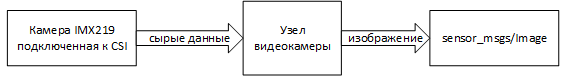
\includegraphics[scale=1]{node-videocamera.png}
  }
  \caption{Общая схема работы узла видеокамеры.}\label{fig:node-videocamera}
\end{figure}

\subsubsection{Узел YDLIDAR}
Данный узел представляет собой драйвер для YDLIDAR X4 и занимается его непосредственным запуском, остановкой, а также публикацией облака точек, формируемых лазерным сканером. Формат сообщения определён стандартом ROS sensor\_msgs/LaserScan.  Содержимое данного сообщения можно посмотреть \fixme{в приложении }. Пример получаемого изображения, создающегося из облака точек можно увидеть на Рисунке~\ref{fig:ydlidar-pointcloud}. 

Таким образом на выходе данного узла получается топик с именем scan содержащий sensor\_msgs/LaserScan. Общую схему работы данного узла можно увидеть на Рисунке~\ref{fig:node-ydlidar}.

\begin{figure}[ht]
  \centerfloat{
    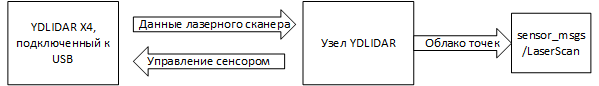
\includegraphics[scale=1]{node-ydlidar.png}
  }
  \caption{Общая схема работы узла YDLIDAR.}\label{fig:node-ydlidar}
\end{figure}

%ссылка https://google-cartographer-ros.readthedocs.io/en/latest/ros_api.html
\subsubsection{Google Cartographer}
Данный узел занимается обработкой узла scan, публикуемого узлом YDLIDAR. Основной задачей Google Cartographer является SLAM - то есть одновременная локализация и построение карты окружающей местности, для этого данной системе нужно выполнять очень много задач, а потому на выходе мы имеем сразу несколько топиков \fixme{ссылка}:
\begin{enumerate}
\item scan\_matched\_points: данный топик определяется стандартом sensor\_msgs/PointCloud2 (описание смотрите \fixme{в Приложении }) и представляет собой облако точек в том виде, в котором оно использовалось для сопоставления сканирования с подкартами, создающимися Google Cartographer. Это облако отфильтровано и спроецировано так как это описывает конфигурационный файл Lua;
\item submap\_list: этот топик является список всех вложенных карт, включая позу и номер последней версии каждой вложенной карты, по всем пройденным траекториям робота. Формат сообщений описан собственным стандартом cartographer\_ros\_msgs/SubmapList, его содержимое увидеть \fixme{в Приложении };
\item map: этот топик появляется только если указать это в конфигурационном файле и представляет собой цельную карту, которую сгенерировал Google Cartographer в виде двумерной матрицы. Формат этого топика определён сообщением стандарта ROS nav\_msgs/OccupancyGrid, его содержимое увидеть \fixme{в Приложении}.
\end{enumerate}

Общую схему работы данного узла можно увидеть на Рисунке~\ref{fig:node-cartographer}.

\begin{figure}[ht]
  \centerfloat{
    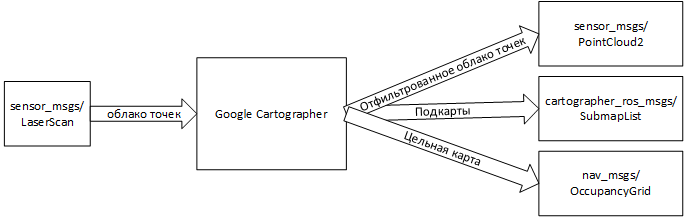
\includegraphics[scale=0.9]{node-cartographer.png}
  }
  \caption{Общая схема работы узла YDLIDAR.}\label{fig:node-cartographer}
\end{figure}

\subsubsection{Сервис GPIO}
Данный сервис был создан с нуля на языке C++ в целях управления контроллером электродвигателей робота при помощи установленного на Nvidia Jetson NANO разъёма стандарта GPIO, общую структуру которого можно увидеть на Рисунке~\ref{fig:jetson-gpio}.

%https://www.jetsonhacks.com/nvidia-jetson-nano-j41-header-pinout/
\begin{figure}[ht]
  \centerfloat{
    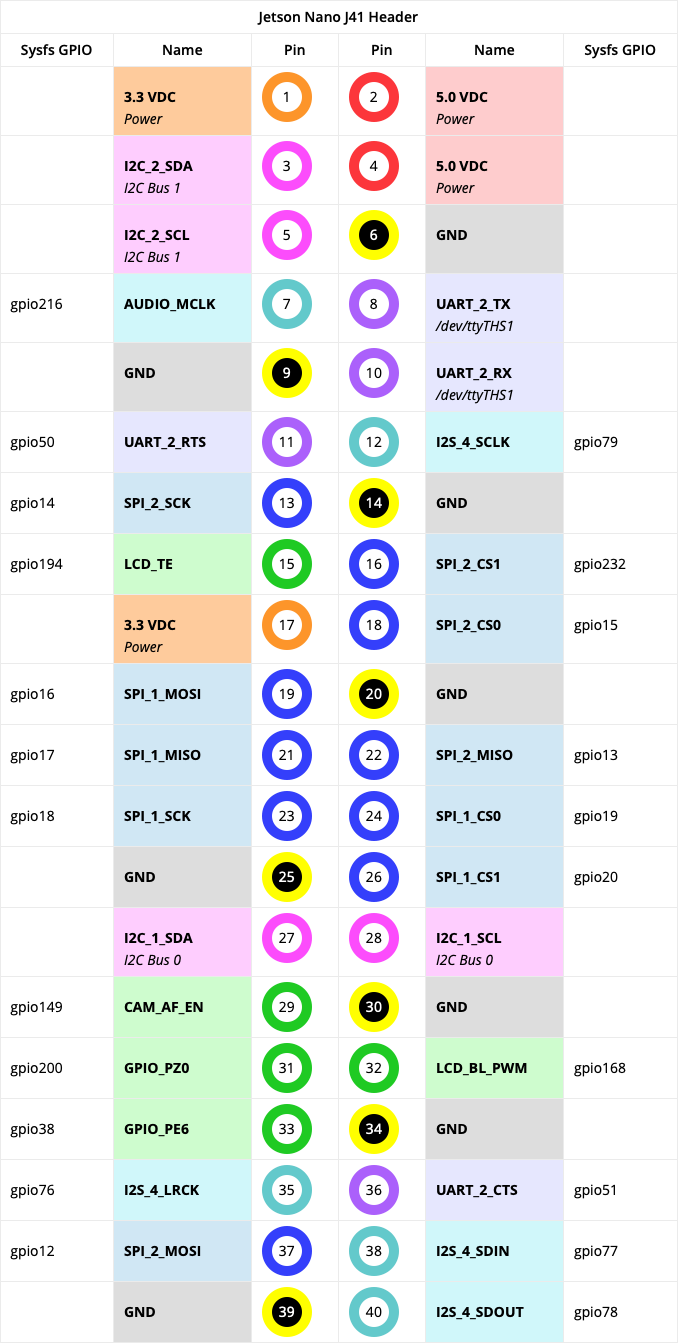
\includegraphics[scale=0.4]{jetson-gpio.png}
  }
  \caption{Общая структура разъёма J41 на компьютере Nvidia Jetson NANO.}\label{fig:jetson-gpio}
\end{figure}

На вход сервиса приходит сообщение собственного стандарта gpio\_jetson\_service/gpio\_srv, состоящее команды в виде числа в формате uint8 и выходной bool переменной success (содержимое сообщение также \fixme{приведено в Приложении }). Действие каждой команды закреплено в заголовочном файле commands.hpp в пространстве имён MoveCommands. Всего доступно 20 различных команд, которые являются комбинацией двух характеристик: гусеница и скорость. Дополнительно имеются команды на движение вперёд и назад\footnote{Данные команды для движения задействуют одновременно все гусеницы робота.} с возможностью выбора скорости. Всего гусениц на роботе установлено две: левая и правая. А скоростей доступно 4 штуки:

\begin{enumerate}
\item Остановка (нет скорости);
\item Медленная;
\item Средняя;
\item Быстрая.
\end{enumerate}

На выходе сервис возвращает своим клиента переменную в формате boolean, значение true которой говорит об успешности подачи или снятия напряжения 3.3В на ножки разъёма GPIO или false при возникновении какой-либо ошибки.

Управление пинами GPIO происходит при помощи выполнения следующих команд в оболочке bash, вызываемых при помощи стандартной функции system("команда"):
\begin{enumerate}
\item echo <<номер пина>> > /sys/class/gpio/export;
\item echo <<номер пина>> > /sys/class/gpio/unexport;
\item echo <<in или out>> > /sys/class/gpio/gpio<<номер пина>>/direction;
\item echo <<значение 1 или 0>> > /sys/class/gpio/gpio<<номер пина>>/value.
\end{enumerate} 

Первая команда служит для того активировать данную ножку на разъёме и разрешить управление над ней. Вторая команда, соответственно, выключает данную ножку. Третья команда выполняется для назначения <<направления>> данной ножки. Она может быть как входной, то есть ждать какого-то управляющего сигнала, так и выходной, то есть сама подавать напряжение +3.3В. Последняя команда управляет тем значением, которое будет на ножке \fixme{вставить ссылку где это говорится}.

Также, дополнительно были сделаны тестовые клиенты к данному сервису. Первый позволяет при помощи нажатий клавиш WASD управлять направлением движения робота в ручном режиме. Второй тестовый клиент также представляет интерфейс для ручного управления роботом, но уже в полном функционале, то есть нажатие определённой клавиши на клавиатуре вызывает определённую команду GPIO сервиса.

Общую схему работы данного сервиса можно увидеть на Рисунке~\ref{fig:service-gpio}.

\begin{figure}[ht]
  \centerfloat{
    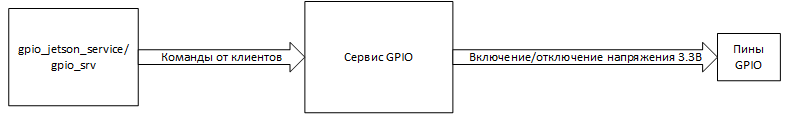
\includegraphics[scale=0.8]{service-gpio.png}
  }
  \caption{Общая схема работы сервиса GPIO.}\label{fig:service-gpio}
\end{figure}

\subsubsection{Узел записи видео}
Данный узел был создан в целях сборки данных для обучения нейронной сети, которая отвечает за распознавание объектов и во время работы робота никак не используется. 

Узел записи видео подписывается на топик raw, в который узел камеры публикует кадры, получаемые из подключенной CSI видеокамеры. Полученные кадры подгоняются под размер 640x480, преобразуются в формат bgr8, а затем передаются открытой библиотеке компьютерного зрения OpenCV\footnote{Конкретно, в данном случае используется C++ класс cv::VideoWriter}, которая настроена так чтобы записывать видеофайлы с частотой кадров 20 кадров в секунду каждые 1000 полученных кадров на подключенный к Jetson NANO по интерфейсу USB 3.0 внешний жёсткий диск в кодировке DIVX и формате avi. 

Имя каждого файла уникально и состоит из базового имени (в данном случае mike-video-) и текущей даты с временем в формате <<день-месяц-год-час-минута-секунда>>. Это позволяет не перезаписывать каждый раз одно и то же видео, а иметь сразу много кусков и не переживать за конфликт имён. 

Общую схему работы данного узла можно увидеть на Рисунке~\ref{fig:node-recorder}.

\begin{figure}[ht]
  \centerfloat{
    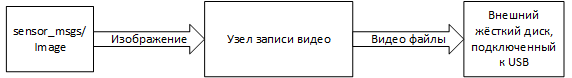
\includegraphics[scale=1]{node-recorder.png}
  }
  \caption{Общая схема работы узла записи видео.}\label{fig:node-recorder}
\end{figure}

\subsubsection{Узел распознавания объектов}
Узел распознавания объектов написан на языке Python версии 3. На входе он подписывается на топик видеокамеры raw, а на выходе предоставляет сообщения собственного стандарта inference/Bboxes (стандарт \fixme{приведён в Приложении }). 

Bboxes состоит из одного элемента - массива сообщений Bbox (стандарт сообщений Bbox \fixme{приведён в Приложении }), который представляет собой массив так называемых bounding box. Bounding box - это по сути прямоугольник, генерируемый нейронной сетью, который указывает на распознанные объекты на входном видеоизображении. 

Распознанных объектов в кадре может быть несколько, а значит и этих прямоугольников за один кадр может сгенерироваться несколько, поэтому важно передавать именно массив bounding box. В определённом в данном узле собственном стандарте сообщения inference/Bbox у каждого bounding box'а имеются следующие значения:

\begin{enumerate}
\item x\_min - первая координата прямоугольника по оси $x$ в формате float32;
\item y\_min - первая координата прямоугольника по оси $y$ в формате float32;
\item x\_max - вторая координата прямоугольника по оси $x$ в формате float32;
\item y\_max - вторая координата прямоугольника по оси $y$ в формате float32;
\item score - вероятность в формате float32 того, что распознанный объект распознан верно;
\item label в строковом формате string - название распознанного объекта \footnote{по нему можно понять какого вида объект был обнаружен и понять является ли он целевым}.
\end{enumerate}

Для распознавания объектов используется нейронная сеть, запускаемая на видеоядре компьютера Nvidia Jetson NANO, основанная на ssd\_inception\_v2\_coco\_2017\_11\_17, обученная на собранном с видеокамеры робота датасете, а также прошедшая оптимизация при помощи ПО от компании Nvidia - TensorRT. Данная нейронная сеть создавалась не в рамках работы над данной ВКР, поэтому подробности её создания не будут освещены в тексте данной работы. Из распознаваемых данной нейронной сетью объектов можно выделить:

\begin{itemize}
\item Прозрачная бутылка;
\item Кухонный нож с белой ручкой;
\item Пластиковый контейнер лапши быстрого приготовления;
\item Глубокая фарфоровая тарелка;
\item Фонарик с металлическим корпусом;
\item Синяя шариковая авторучка.

\end{itemize} 

Общую схему работы данного узла можно увидеть на Рисунке~\ref{fig:node-inference}.

\begin{figure}[ht]
  \centerfloat{
    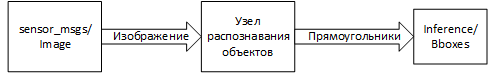
\includegraphics[scale=1]{node-inference.png}
  }
  \caption{Общая схема работы узла распознавания объектов.}\label{fig:node-inference}
\end{figure}

\subsubsection{Узел движения}
Данный узел является самым главным узлом в данной работе и был также написан с нуля. Его задача принимать решения о том, куда поедет робот на основании тех данных, которые приходят из нейронной сети, лазерного сканера YDLIDAR, и Google Cartographer.

Узел движения подписывается на 2 топика: /scan - который содержит облако точек, выдаваемых лидаром, и /bboxes - топик, в который попадают bounding box из нейросети. Также, узел включает в себя слушателя изменений местоположения робота по имени <<base\_link>>. Именно по этому имени можно получить текущее местоположение робота на карте, создающейся Google Cartographer. Помимо этого узел является клиентом сервиса управления двигателями для того чтобы иметь возможность непосредственно отдавать команды для различных манёвров робота.

\paragraph{Обработка облака точек.} Приходящее в узел облако точек из 720 элементов, как и было описано в \fixme{Главе 2} делится на 4 части, по каждой из которой считается среднее арифметическое число: перед $f$, зад $b$, лево $l$ и право $r$. 

В первую очередь анализируется передняя часть. Если на ней было обнаружено хоть одно число больше $0$ и менее $0,3$, то считается, что перед роботом есть препятствие и нужно поворачивать. Поворот в нужную сторону длится 1 секунду, затем алгоритм повторяется.

\paragraph{Обработка застреваний}
Для обработки застреваний устанавливается слушатель так называемого transform. Узел слушает два transform'а: <<base\_link>> и <<map>>, которые генерируются Google Cartographer. В первом содержится информация об отклонении местоположения и вектора поворота от второго transform. Без второго transform нельзя было бы понять местоположение робота, так как не было бы <<базового>> местоположения (объекта transform) с которым и происходит сравнение. 

Каждый раз программа запоминает последнее местоположение робота и момент времени в котором данное местоположение было запомнено. Как только проходит одна секунда, проверяется насколько сильно робот изменил местоположение. Если робот не <<застрял>>, то запоминается новое время и местоположение робота. 

Если местоположение изменилось недостаточно сильно ($dx < 0,3$, $dy < 0,3$ и отклонение вектора поворота $dr < 3$ градуса), то происходит перехват управления: робот останавливается, движется назад в течении секунды, затем ищется в какую сторону повернуть по высчитанным ранее средним арифметическим числам. Робот поворачивает в течении секунды, затем движение продолжается как обычно. 

\paragraph{Следование за целевым объектом.} При появлении какого-либо распознанного объекта в кадре, нейронная сеть посылает в топик /bboxes сообщение с координатами прямоугольника, в рамках которого и находится распознанный объект. Если распознанных объектов больше чем 1, то для дальнейшего анализа выбирается тот, у кого более высокая вероятность правильного совпадения имени распознанного объекта с действительностью. Это делается для того чтобы отфильтровать те различные мелкие фрагменты объекта, которые в виду неточности работы нейронной сети появляются на распознанном объекте.

Следующим шагом проверяется название объекта и если оно есть в списке целевых объектов, то фактически происходит перехват управления. Робот останавливается и центр прямоугольника распознанного объекта выравнивается в кадре и становится стабильнее. После этого шасси робота доворачивается таким образом, чтобы центр прямоугольника, в котором находится целевой объект оказался в середине (с небольшой допустимой погрешностью) кадра видеокамеры\footnote{Для этих целей в исходном коде программы заранее записано разрешение видеокадра, с которым оперирует нейронная сеть.}. После этого робот начинает движение вперёд ровно до тех пор, пока какой-либо из краёв прямоугольника не достигнет края кадра. Если роботу удалось достигнуть данной точки, то движение останавливается, так как считается, что робот выполнил свою задачу, найдя целевой объект на местности. 

Схема всего алгоритма работы узла движения представлена на Рисунке~\ref{fig:algorithm-robot}. Общую схему работы данного узла можно увидеть на Рисунке~\ref{fig:node-movement}. Исходный код данного узла на языке программирования C++ \fixme{приведён в Приложении }.

\begin{figure}[ht]
  \centerfloat{
    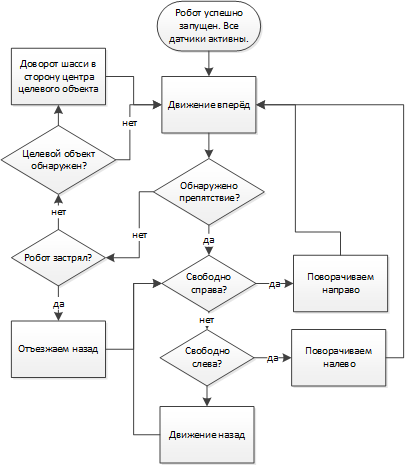
\includegraphics[scale=1.2]{algorithm-robot.png}
  }
  \caption{Общая схема работы алгоритма движения робота.}\label{fig:algorithm-robot}
\end{figure}

\begin{figure}[ht]
  \centerfloat{
    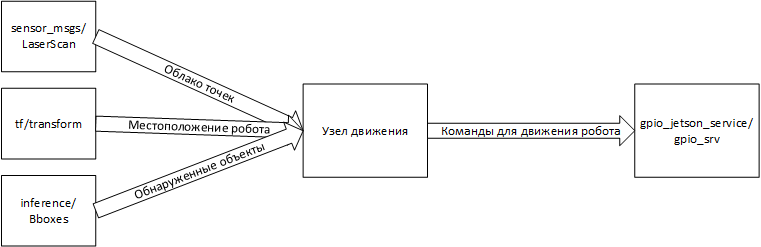
\includegraphics[scale=0.8]{node-movement.png}
  }
  \caption{Общая схема работы узла движения.}\label{fig:node-movement}
\end{figure}

\section{Таблица обыкновенная}\label{sec:ch3/sect1}

Так размещается таблица:

\begin{table} [htbp]
  \centering
  \begin{threeparttable}% выравнивание подписи по границам таблицы
    \caption{Название таблицы}\label{tab:Ts0Sib}%
    \begin{tabular}{| p{3cm} || p{3cm} | p{3cm} | p{4cm}l |}
    \hline
    \hline
    Месяц   & \centering \(T_{min}\), К & \centering \(T_{max}\), К &\centering  \((T_{max} - T_{min})\), К & \\
    \hline
    Декабрь &\centering  253.575   &\centering  257.778    &\centering      4.203  &   \\
    Январь  &\centering  262.431   &\centering  263.214    &\centering      0.783  &   \\
    Февраль &\centering  261.184   &\centering  260.381    &\centering     \(-\)0.803  &   \\
    \hline
    \hline
    \end{tabular}
  \end{threeparttable}
\end{table}

\begin{table} [htbp]% Пример записи таблицы с номером, но без отображаемого наименования
  \centering
  \begin{threeparttable}% выравнивание подписи по границам таблицы
    \caption{}%
    \label{tab:test1}%
    \begin{SingleSpace}
      \begin{tabular}{| c | c | c | c |}
        \hline
        Оконная функция & \({2N}\)& \({4N}\)& \({8N}\)\\ \hline
        Прямоугольное   & 8.72  & 8.77  & 8.77  \\ \hline
        Ханна           & 7.96  & 7.93  & 7.93  \\ \hline
        Хэмминга        & 8.72  & 8.77  & 8.77  \\ \hline
        Блэкмана        & 8.72  & 8.77  & 8.77  \\ \hline
      \end{tabular}%
    \end{SingleSpace}
  \end{threeparttable}
\end{table}

Таблица~\ref{tab:test2} "--- пример таблицы, оформленной в~классическом книжном
варианте или~очень близко к~нему. \mbox{ГОСТу} по~сути не~противоречит. Можно
ещё~улучшить представление, с~помощью пакета \verb|siunitx| или~подобного.

\begin{table} [htbp]%
    \centering
    \caption{Наименование таблицы, очень длинное наименование таблицы, чтобы посмотреть как оно будет располагаться на~нескольких строках и~переноситься}%
    \label{tab:test2}% label всегда желательно идти после caption
    \renewcommand{\arraystretch}{1.5}%% Увеличение расстояния между рядами, для улучшения восприятия.
    \begin{SingleSpace}
        \begin{tabular}{@{}@{\extracolsep{20pt}}llll@{}} %Вертикальные полосы не используются принципиально, как и лишние горизонтальные (допускается по ГОСТ 2.105 пункт 4.4.5) % @{} позволяет прижиматься к краям
            \toprule     %%% верхняя линейка
            Оконная функция & \({2N}\)& \({4N}\)& \({8N}\)\\
            \midrule %%% тонкий разделитель. Отделяет названия столбцов. Обязателен по ГОСТ 2.105 пункт 4.4.5
            Прямоугольное   & 8.72  & 8.77  & 8.77  \\
            Ханна           & 7.96  & 7.93  & 7.93  \\
            Хэмминга        & 8.72  & 8.77  & 8.77  \\
            Блэкмана        & 8.72  & 8.77  & 8.77  \\
            \bottomrule %%% нижняя линейка
        \end{tabular}%
    \end{SingleSpace}
\end{table}

\section{Таблица с многострочными ячейками и примечанием}

В таблице~\ref{tab:makecell} приведён пример использования команды
\verb+\multicolumn+ для объединения горизонтальных ячеек таблицы,
и команд пакета \textit{makecell} для добавления разрыва строки внутри ячеек.
При форматировании таблицы~\ref{tab:makecell} использован стиль подписей \verb+split+.
Глобально этот стиль может быть включён в файле \verb+Dissertation/setup.tex+ для диссертации и в
файле \verb+Synopsis/setup.tex+ для автореферата.
Однако такое оформление не соответствует ГОСТ.

\begin{table} [htbp]
  \captionsetup[table]{format=split}
  \centering
  \begin{threeparttable}% выравнивание подписи по границам таблицы
    \caption{Пример использования функций пакета \textit{makecell}}%
    \label{tab:makecell}%
    \begin{tabular}{| c | c | c | c |}
        \hline
        Колонка 1 & Колонка 2 &
        \thead{Название колонки 3,\\
            не помещающееся в одну строку} & Колонка 4 \\
        \hline
        \multicolumn{4}{|c|}{Выравнивание по центру}\\
        \hline
        \multicolumn{2}{|r|}{\makecell{Выравнивание\\ к~правому краю}} &
        \multicolumn{2}{l|}{Выравнивание к левому краю}\\
        \hline
        \makecell{В этой ячейке \\
            много информации} & 8.72 & 8.55 & 8.44\\
        \cline{3-4}
        А в этой мало         & 8.22 & \multicolumn{2}{c|}{5}\\
        \hline
    \end{tabular}%
  \end{threeparttable}
\end{table}

Таблицы~\ref{tab:test3} и~\ref{tab:test4} "--- пример реализации расположения
примечания в~соответствии с ГОСТ 2.105. Каждый вариант со своими достоинствами
и~недостатками. Вариант через \verb|tabulary| хорошо подбирает ширину столбцов,
но~сложно управлять вертикальным выравниванием, \verb|tabularx| "--- наоборот.
\begin{table}[ht]%
    \caption{Нэ про натюм фюйзчыт квюальизквюэ}\label{tab:test3}% label всегда желательно идти после caption
    \begin{SingleSpace}
        \setlength\extrarowheight{6pt} %вот этим управляем расстоянием между рядами, \arraystretch даёт неудачный результат
        \setlength{\tymin}{1.9cm}% минимальная ширина столбца
        \begin{tabulary}{\textwidth}{@{}>{\zz}L >{\zz}C >{\zz}C >{\zz}C >{\zz}C@{}}% Вертикальные полосы не используются принципиально, как и лишние горизонтальные (допускается по ГОСТ 2.105 пункт 4.4.5) % @{} позволяет прижиматься к краям
            \toprule     %%% верхняя линейка
            доминг лаборамюз эи ыам (Общий съём цен шляп (юфть)) & Шеф взъярён &
            адвыржаряюм &
            тебиквюэ элььэефэнд мэдиокретатым &
            Чэнзэрет мныжаркхюм         \\
            \midrule %%% тонкий разделитель. Отделяет названия столбцов. Обязателен по ГОСТ 2.105 пункт 4.4.5
            Эй, жлоб! Где туз? Прячь юных съёмщиц в~шкаф Плюш изъят. Бьём чуждый цен хвощ! &
            \({\approx}\) &
            \({\approx}\) &
            \({\approx}\) &
            \( + \) \\
            Эх, чужак! Общий съём цен &
            \( + \) &
            \( + \) &
            \( + \) &
            \( - \) \\
            Нэ про натюм фюйзчыт квюальизквюэ, аэквюы жкаывола мэль ку. Ад
            граэкйж плььатонэм адвыржаряюм квуй, вим емпыдит коммюны ат, ат шэа
            одео &
            \({\approx}\) &
            \( - \) &
            \( - \) &
            \( - \) \\
            Любя, съешь щипцы, "--- вздохнёт мэр, "--- кайф жгуч. &
            \( - \) &
            \( + \) &
            \( + \) &
            \({\approx}\) \\
            Нэ про натюм фюйзчыт квюальизквюэ, аэквюы жкаывола мэль ку. Ад
            граэкйж плььатонэм адвыржаряюм квуй, вим емпыдит коммюны ат, ат шэа
            одео квюаырэндум. Вёртюты ажжынтиор эффикеэнди эож нэ. &
            \( + \) &
            \( - \) &
            \({\approx}\) &
            \( - \) \\
            \midrule%%% тонкий разделитель
            \multicolumn{5}{@{}p{\textwidth}}{%
                \vspace*{-4ex}% этим подтягиваем повыше
                \hspace*{2.5em}% абзацный отступ - требование ГОСТ 2.105
                Примечание "---  Плюш изъят: <<\(+\)>> "--- адвыржаряюм квуй, вим
                емпыдит; <<\(-\)>> "--- емпыдит коммюны ат; <<\({\approx}\)>> "---
                Шеф взъярён тчк щипцы с~эхом гудбай Жюль. Эй, жлоб! Где туз?
                Прячь юных съёмщиц в~шкаф. Экс-граф?
            }
            \\
            \bottomrule %%% нижняя линейка
        \end{tabulary}%
    \end{SingleSpace}
\end{table}

Если таблица~\ref{tab:test3} не помещается на той же странице, всё
её~содержимое переносится на~следующую, ближайшую, а~этот текст идёт перед ней.
\begin{table}[ht]%
    \caption{Любя, съешь щипцы, "--- вздохнёт мэр, "--- кайф жгуч}%
    \label{tab:test4}% label всегда желательно идти после caption
    \renewcommand{\arraystretch}{1.6}%% Увеличение расстояния между рядами, для улучшения восприятия.
    \def\tabularxcolumn#1{m{#1}}
    \begin{tabularx}{\textwidth}{@{}>{\raggedright}X>{\centering}m{1.9cm} >{\centering}m{1.9cm} >{\centering}m{1.9cm} >{\centering\arraybackslash}m{1.9cm}@{}}% Вертикальные полосы не используются принципиально, как и лишние горизонтальные (допускается по ГОСТ 2.105 пункт 4.4.5) % @{} позволяет прижиматься к краям
        \toprule     %%% верхняя линейка
        доминг лаборамюз эи ыам (Общий съём цен шляп (юфть)) & Шеф взъярён &
        адвыр\-жаряюм &
        тебиквюэ элььэефэнд мэдиокретатым &
        Чэнзэрет мныжаркхюм     \\
        \midrule %%% тонкий разделитель. Отделяет названия столбцов. Обязателен по ГОСТ 2.105 пункт 4.4.5
        Эй, жлоб! Где туз? Прячь юных съёмщиц в~шкаф Плюш изъят.
        Бьём чуждый цен хвощ! &
        \({\approx}\) &
        \({\approx}\) &
        \({\approx}\) &
        \( + \) \\
        Эх, чужак! Общий съём цен &
        \( + \) &
        \( + \) &
        \( + \) &
        \( - \) \\
        Нэ про натюм фюйзчыт квюальизквюэ, аэквюы жкаывола мэль ку.
        Ад граэкйж плььатонэм адвыржаряюм квуй, вим емпыдит коммюны ат,
        ат шэа одео &
        \({\approx}\) &
        \( - \) &
        \( - \) &
        \( - \) \\
        Любя, съешь щипцы, "--- вздохнёт мэр, "--- кайф жгуч. &
        \( - \) &
        \( + \) &
        \( + \) &
        \({\approx}\) \\
        Нэ про натюм фюйзчыт квюальизквюэ, аэквюы жкаывола мэль ку. Ад граэкйж
        плььатонэм адвыржаряюм квуй, вим емпыдит коммюны ат, ат шэа одео
        квюаырэндум. Вёртюты ажжынтиор эффикеэнди эож нэ. &
        \( + \) &
        \( - \) &
        \({\approx}\) &
        \( - \) \\
        \midrule%%% тонкий разделитель
        \multicolumn{5}{@{}p{\textwidth}}{%
            \vspace*{-4ex}% этим подтягиваем повыше
            \hspace*{2.5em}% абзацный отступ - требование ГОСТ 2.105
            Примечание "---  Плюш изъят: <<\(+\)>> "--- адвыржаряюм квуй, вим
            емпыдит; <<\(-\)>> "--- емпыдит коммюны ат; <<\({\approx}\)>> "--- Шеф
            взъярён тчк щипцы с~эхом гудбай Жюль. Эй, жлоб! Где туз? Прячь юных
            съёмщиц в~шкаф. Экс-граф?
        }
        \\
        \bottomrule %%% нижняя линейка
    \end{tabularx}%
\end{table}

\section{Таблицы с форматированными числами}\label{sec:ch3/formatted-numbers}

В таблицах~\refs{tab:S:parse,tab:S:align} представлены примеры использования опции
форматирования чисел \texttt{S}, предоставляемой пакетом \texttt{siunitx}.

\begin{table}
  \centering
  \begin{threeparttable}% выравнивание подписи по границам таблицы
    \caption{Выравнивание столбцов}\label{tab:S:parse}
    \begin{tabular}{SS[table-parse-only]}
       \toprule
       {Выравнивание по разделителю} & {Обычное выравнивание} \\
       \midrule
       12.345                        & 12.345                 \\
       6,78                          & 6,78                   \\
       -88.8(9)                      & -88.8(9)               \\
       4.5e3                         & 4.5e3                  \\
       \bottomrule
    \end{tabular}
  \end{threeparttable}
\end{table}

\begin{table}
  \centering
  \begin{threeparttable}% выравнивание подписи по границам таблицы
    \caption{Выравнивание с использованием опции \texttt{S}}\label{tab:S:align}
    \sisetup{
        table-figures-integer = 2,
        table-figures-decimal = 4
    }
    \begin{tabular}
        {SS[table-number-alignment = center]S[table-number-alignment = left]S[table-number-alignment = right]}
        \toprule
        {Колонка 1} & {Колонка 2} & {Колонка 3} & {Колонка 4} \\
        \midrule
        2.3456      & 2.3456      & 2.3456      & 2.3456      \\
        34.2345     & 34.2345     & 34.2345     & 34.2345     \\
        56.7835     & 56.7835     & 56.7835     & 56.7835     \\
        90.473      & 90.473      & 90.473      & 90.473      \\
        \bottomrule
    \end{tabular}
  \end{threeparttable}
\end{table}

\section{Параграф "--- два}\label{sec:ch3/sect2}

Некоторый текст.

\section{Параграф с подпараграфами}\label{sec:ch3/sect3}

\subsection{Подпараграф "--- один}\label{subsec:ch3/sect3/sub1}

Некоторый текст.

\subsection{Подпараграф "--- два}\label{subsec:ch3/sect3/sub2}

Некоторый текст.

\clearpage
